%  article.tex (Version 3.3, released 19 January 2008)
%  Article to demonstrate format for SPIE Proceedings
%  Special instructions are included in this file after the
%  symbol %>>>>
%  Numerous commands are commented out, but included to show how
%  to effect various options, e.g., to print page numbers, etc.
%  This LaTeX source file is composed for LaTeX2e.

%  The following commands have been added in the SPIE class 
%  file (spie.cls) and will not be understood in other classes:
%  \supit{}, \authorinfo{}, \skiplinehalf, \keywords{}
%  The bibliography style file is called spiebib.bst, 
%  which replaces the standard style unstr.bst.  

\documentclass[]{spie}  %>>> use for US letter paper
%%\documentclass[a4paper]{spie}  %>>> use this instead for A4 paper
%%\documentclass[nocompress]{spie}  %>>> to avoid compression of citations
%% \addtolength{\voffset}{9mm}   %>>> moves text field down
%% \renewcommand{\baselinestretch}{1.65}   %>>> 1.65 for double spacing, 1.25 for 1.5 spacing 
%  The following command loads a graphics package to include images 
%  in the document. It may be necessary to specify a DVI driver option,
%  e.g., [dvips], but that may be inappropriate for some LaTeX 
%  installations. 
\usepackage[]{graphicx}
\usepackage{epstopdf}

\title{Using DARC in a Multi-Object AO Bench and in a Dome Seeing Instrument}

%>>>> The author is responsible for formatting the 
%  author list and their institutions.  Use  \skiplinehalf 
%  to separate author list from addresses and between each address.
%  The correspondence between each author and his/her address
%  can be indicated with a superscript in italics, 
%  which is easily obtained with \supit{}.

\author{Norman S\'aez$\supit{a}^{*}$, Alastair Basden\supit{b}, Dani Guzm\'an\supit{a}, Nicol\'as Dubost\supit{a}
\skiplinehalf
\supit{a}Pontificia Universidad Cat\'olica de Chile, Centre for Astro-Engineering, Av.Vicu\~na Mackenna 4860, Santiago, Chile\\
\supit{b}University of Durham, Department of Physics, Centre for Advanced Instrumentation, South Road, Durham DH1 3LE, UK\\ $*$nfsaez@uc.cl
%\supit{b}Affiliation2, Address, City, Country
}

%>>>> Further information about the authors, other than their 
%  institution and addresses, should be included as a footnote, 
%  which is facilitated by the \authorinfo{} command.

\authorinfo{Further author information: Norman S\'aez: E-mail: nfsaez@uc.cl}
%%>>>> when using amstex, you need to use @@ instead of @
 

%%%%%%%%%%%%%%%%%%%%%%%%%%%%%%%%%%%%%%%%%%%%%%%%%%%%%%%%%%%%% 
%>>>> uncomment following for page numbers
% \pagestyle{plain}    
%>>>> uncomment following to start page numbering at 301 
%\setcounter{page}{301} 
 
  \begin{document} 
  \maketitle 

%%%%%%%%%%%%%%%%%%%%%%%%%%%%%%%%%%%%%%%%%%%%%%%%%%%%%%%%%%%%% 
\begin{abstract}
The Durham adaptive Optics Real Time Controller (DARC)\cite{basden2010durham}
is a real-time system for astronomical adaptive optics systems originally
developed at Durham University and in use for the CANARY instrument. One of its
main strengths is to be a generic and high performance real-time controller
running on an off-the-shelf Linux computer. DARC is an open-source project. We
are using DARC for two different implementations: BEAGLE, a Multi-Object AO
(MOAO) bench system to experiment with novel tomographic reconstructors and
LOTUCE2, an in-dome turbulence instrument. We present the software architecture
for each application, current benchmarks and lessons learned for current and
future DARC developers.
\end{abstract}

%>>>> Include a list of keywords after the abstract 

\keywords{DARC, Adaptive Optics,  Multi-Object Adaptive Optics, real-time control, Charge Coupled Device}

%%%%%%%%%%%%%%%%%%%%%%%%%%%%%%%%%%%%%%%%%%%%%%%%%%%%%%%%%%%%%
\section{INTRODUCTION}\label{sec:intro}  % \label{} allows reference to this section
The Durham adaptive Optics Real Time Controller (DARC) is a real-time system
for astronomical adaptive optics systems originally developed at Durham
University and in use for the CANARY instrument. One of its main strengths is
to be a generic and high performance real-time controller running on an
off-the-shelf Linux computer. It was developed in a modular way making it
flexible enough for simple or sophisticated AO instruments. Very importantly,
DARC is an open-source project. Taking advantage of its modularization degree,
it is possible to implement different AO algorithms as well as different pieces
of hardware, such as cameras for wavefront sensors (WFS) and deformable
mirrors. As it is a standard Linux application, it is possible to take
advantage of external components which can be interfaced in Linux, such as
fire-wire or GigE cameras. For new components, it is always possible to build a
Linux driver and Application Program Interface that can control the device.
DARC uses currently multi-core technologies efficiently, performing at speeds
that were only possible to achieve with complex architectures in the past\cite{basden2012durham}. 
We are using DARC for two different implementations: BEAGLE and LOTUCE2. BEAGLE
(presented elsewhere at this conference) is a Multi-Object AO (MOAO) bench
system to experiment with novel tomographic reconstructors, such as Artificial
Neural Networks. For BEAGLE we have developed a new module within DARC, which
runs the bench in a ``multiple WFS'' mode, by controlling a constellation of light
sources, three phase plates mechanisms and only one WFS camera. DARC runs this
system in conjunction with a Single Board Computer which is in charge of some
of the hardware components. LOTUCE2 (presented elsewhere at this conference) is
an in-dome turbulence instrument, which measures the angle-of-arrival of
multiple lasers to individual high-speed cameras. DARC has been used to run
four cameras, which have in-sync a hardware trigger. DARC processes the pixel
streams, obtaining the angle-of-arrival from each camera, saving data to disk
and performing various analysis in real-time. We present the software
architecture for each application, current benchmarks and lessons learned for
current and future DARC developers.

\subsection{BEAGLE}
BEAGLE is a Multi-Object AO (MOAO) bench that can emulate the optical
characteristics of the William Hershel Telescope, it has two motorized phase
plates which allow to change the position of the plate scale. DARC, a real-time
system for astronomical adaptive optics systems, is being used to control
acquisition images. Extra development was necessary in order to integrate specific hardware
device components which represent phase plate movement and guide stars. The
main features which DARC provides which BEAGLE uses are the centroid calculation
in real-time\cite{basden2012wavefront}, and camera control for the fire-wire
protocol. It was pending to create a way to controls new peripherals
to make BEAGLE work. To meet this objective, a single board computer was used.
The selected single board computer was a Beagle Bone Back (BBB). The challenge
of integrating DARC with the new single board computer was relatively simple, and
relied on a local area network (TCP/IP connectivity) and a scripting language
as glue. 


\subsection{LOTUCE2}
Lotuce (LOcal Turbulence Experiment)\cite{ziad1a2013lotuce} is an experimental
concept to measure and characterize the optical-turbulence inside a telescope
enclosure\cite{berdja1afirst}. LOTUCE2 is an upgraded
prototype whose main aim is to measure optical turbulence characteristics more
precisely by minimizing cross-contamination of signals. This characterization
is both quantitative (optical turbulence strength) and qualitative (assessing
        the optical turbulence statistical model). 
% in order to measure and characterize the so-called dome-seeing.


\section{Software Architecture}\label{sec:SWA} 
The Durham AO real-time controller (DARC) is composed of several software
components: The real-time control pipeline (RTCP), control, diagnostic and
graphical modules, background tasks, and a scripting interface. The RTCP's main
task is taking data from cameras (WFS) and computing control vectors to be sent
to deformable mirrors. The control interface allows updates and controls RTCP.
The diagnostic module takes the output from the RTCP for debugging purposes.
Graphical and scripting interfaces allow the user to interact with the whole
system through the control interface\cite{basden2010durham}.


\subsection{BEAGLE}
BEAGLE is using DARC to control acquisition images (controlling a camera with
a fire-wire protocol) and centroid calculations in real-time, mainly RTCP.
Extra development was necessary to integrate specific hardware device components.
BEAGLE has to integrate phase plate movements (motors) and guide stars
(leds). To fulfill this objective, a single board computer was used. The selected
single board computer was a Beagle Bone Back (BBB).  The challenge of
integrating DARC with the new single board computer was relatively simple, and
relied on a local area network (TCP/IP connectivity) and scripting.  

 In order to follow the same paradigms of DARC, an omniORB was installed in
 the BBB. This let to develop a CORBA server, which controls most of the
 peripherals in the BBB. Real time software is not required in the BBB, due to
 acquisition methods.  For the BBB CORBA server, the Python language was used.
 The BBB has general-purpose input/output (GPIO) pins which are connected to
 motors and leds(phase plate and stars respectively). The BBB Server listens to
 requirements, and each requirement controls a specific GPIO pin. The BBB has
 its own python    libraries to controls GPIO pins, and is called adafruit, but
 the    performance on motors  was not good enough.   To improve the behaviour
 a    C-Python extension was developed. The C-Python extension is imported as a
 standard python module and is used in the BBB Server with no significant
 modifications.

As was explained before, DARC makes it possible to change the system's behaviour
by using a scripting and a control interface. The BBB Server is able to communicate with
a host connected to a reachable IP address. Therefore, the communication
between DARC and the BBB Server is straightforward. DARC is currently installed in a
powerful machine called RTCAOLAB; figure [\ref{fig:phy_lay}] shows the physical
layout. 

%-------------
   \begin{figure}[!ht]
   \begin{center}
   \begin{tabular}{c}
   \includegraphics[height=4.0cm]{../img/physical_layout.jpg}
   \end{tabular}
   \end{center}
   \caption[phy] 
   { \label{fig:phy_lay} BEAGLE physical layout connections}
   \end{figure} 
%-------------

Using mostly a script interface, it is possible to build an entire class model on
the top. RTCAOLAB was used as a ``central server'', in this way, setup routines,
    calibration scripts, phase plate, guide stars are controlled using only
    this host. From a user point of view, it is completely transparent which host
    is in charge of which device. Figure [\ref{fig:class}] shows the complete class
    model built on the top.

%-------------
   \begin{figure}[!ht]
   \begin{center}
   \begin{tabular}{c}
   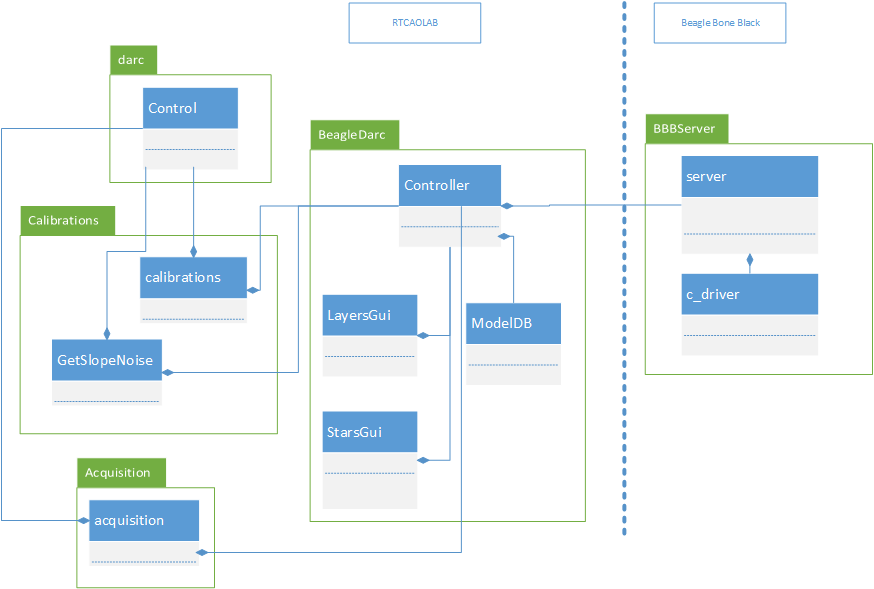
\includegraphics[height=9.0cm]{../img/class_model2.png}
   \end{tabular}
   \end{center}
   \caption[class] 
   { \label{fig:class} BeagleDarc Class Model. White boxes contain host name where those packages are running.}
   \end{figure}
%-------------

\subsection{LOTUCE2}
Lotuce (LOcal Turbulence Experiment) is an experimental to measure and
characterized the optical-turbulence inside a telescope enclosure. LOTUCE2 is
an upgraded prototype whose main aim is to measure optical turbulence
characteristics more precisely by minimizing cross-contamination of signals.
Initially, Lotuce used a single camera, LOTUCE2 instead  uses four cameras.
Camera acquisition and slopes calculation are features provided by DARC.

Replicating a software environment was an item to worry about. In order to be
confident enough that it was possible to replicate the environment, DARC was
installed in two different machines. A Mac Book pro Late2011 and a
Desktop machine are the hosts for DARC's current deployment. Different operating
systems were used, but the same software was compiled on them. The
Desktop machine used a Fedora 14 Linux kernel 2.6.35.13-91 32 bits architecture.
The Mac Book pro instead had installed a Linux Ubuntu 13.10 kernel 3.11.0-15
64bits architecture.  Besides this difference, the behaviour was exactly the
same. Notice that each kernel is not patched as real time, but it was good
enough for LOTUCE2 purposes. It is worth to mention that we are using  Mac Book
pro either Desktop for the following tests with the same results.

DARC is highly flexible with each camera protocol, it can handle USB, ieee1394
cameras (fire-wire cameras) as well as Ethernet Gig protocols. Cameras used a
two Gigabit Ethernet protocol and a Cisco 3560 was configured to plug all possible
cameras. This switch was transparent to DARC for either installation.  

Camera synchronization was a real challenge. The approach taken used an
external trigger shared among the cameras. The device used to trigger the
camera acquisition was a single board computer, integrated and
configurable GPIO pins.  The Beagle Bone Black (BBB) was the selected for these
purposes. The BBB has an ARM Cortex-A8 processor, with a embedded Linux inside.
The embedded Linux flavour is Ubuntu13.10. 100 [KHz] was the  maximum frequency
reached when turning on/off the GPIO pin. To improve this situation, a
programmable real-time unit(PRU) was used.This unit performs embedded tasks
that require real-time constraints. PRU is a subsystem of the processor inside
the BBB. It is an independent CPU with its own memory and instruction set. It
can run its own program, completely independent of the Linux kernel on the main
CPU. Using the PRU approach, the BBB could reach a signal frequency of
200[MHz], meeting LOTUCE2 requirements.

DARC can obtain the data from both cameras in a single stream or each camera in
a separate stream. If the single stream approach is used, the streams stick one
next to the other. It is mandatory that each camera protocol has its own driver
implementation to make it compatible with DARC. Aravis is a library for video
acquisition which is being used to make the driver work in DARC. Using both
cameras at the same time (but not at maximum resolution) we are getting results
up to 200 [fps], which are very promising results. The trigger to obtain images
with the cameras is working fine but is still under testing.Figure
[\ref{fig:lpl}] shows the current layout design. Slight modifications are not
discarded at this time.

%-------------
   \begin{figure}[!ht]
   \begin{center}
   \begin{tabular}{c}
   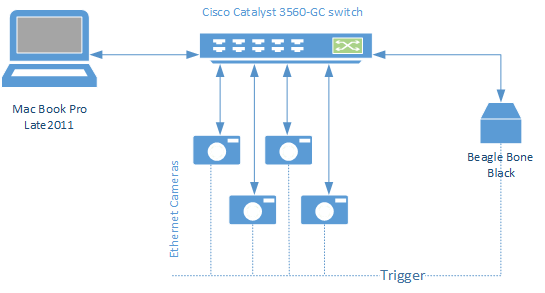
\includegraphics[height=6.0cm]{../img/physical_layout_lotuce.png}
   \end{tabular}
   \end{center}
   \caption[lpl] 
   { \label{fig:lpl} LOTUCE2 physical layout}
   \end{figure} 
%-------------

The main program should be running where DARC is installed (either Mac Book pro
        or Desktop) and the signal trigger it will be send using TCP/IP
protocol, arriving at BBB, triggering the acquisition. Some automatic routines
are being implemented, like automatic sub aperture location, ideal image size
and some graphics plots to help to controls the instrument operations. Image
[\ref{fig:step2}] shows a prototype GUI example. Most of the software modules
and interfaces are still under development.

%-------------
   \begin{figure}[!ht]
   \begin{center}
   \begin{tabular}{c}
   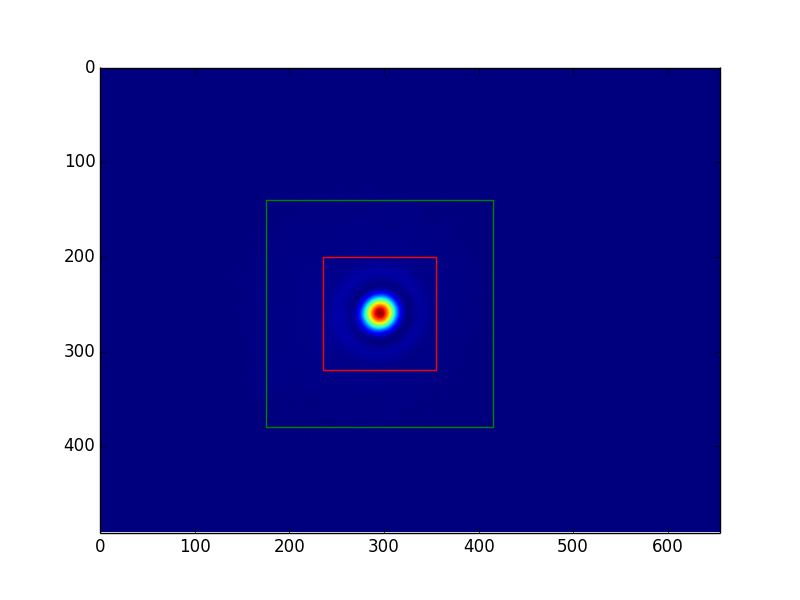
\includegraphics[height=6.0cm]{../img/step2b.png}
   \end{tabular}
   \end{center}
   \caption[step2] 
   { \label{fig:step2} LOTUCE2 interface prototype just after adjust sub aperture location (red) and image size (green)}
   \end{figure} 
%-------------

%%%%%%%%%%%%%%%%%%%%%%%%%%%%%%%%%%%%%%%%%%%%%%%%%%%%%%%%%%%%%
\newpage
\section{Software Development supported by DARC and Experimental Tests Experience} \label{sec:LL}
DARC is written in C and Python, which are languages with strengths and
weaknesses. DARC takes advantage of their strengths making an excellent
combination; C run-time speed and Python fast develop. Most of the current work
has been implemented using DARC CORBA control interface, which let us use fast
scripting development and quick prototypes, through Python. Environment setup,
          calibration routines, repetitive operation and graphical user
          interfaces will be described in this section as well as some
          empirical test experiences.

\subsection{BEAGLE}
Before start to obtain data, BEAGLE bench needs to be prepared and calibrated
properly. Exposure time per each star, background levels, reference centroids
are fundamental to the right bench operation.

In calibration routines, each led (a star) has its own brightest (by
manufacturer). Because of this each one needs its own exposure time and the
corresponding background image. Using an iteration process it is possible get
the best exposure time per each led. Once the best exposure time is reached,
background image is obtained. Once the above process finish, sub apertures are
located using correlation through convolution (no turbulence is present). the
centroid calculations given by DARC can be done after determining all the sub
apertures. Also DARC is set to consider the $n$ brightest pixels within a sub
aperture to calculate centroid.\cite{basden2012wavefront} The $n$ number is
also obtained through iterative process.

The acquisition has two operational modes: phase screen move swiftly to a given
altitude at a regular step and phase screen moves randomly horizontally and
vertically. Using the second mode, its finds the shortest path to reach the
random position, in order to keep acquisition time at minimum. In both cases a
led sequences turn on/off taking images and/or slopes, saving results in fits
files. All led has it own background, sub aperture location, exposure time and
reference centroids as mentioned.

BEAGLE used two ieee1394 cameras simultaneously, and during empirical tests,
one of them got stuck. We realized that the card which both cameras were
plugged, it not given the best bandwidth, it was shared. The solution was given
a dedicated card per each camera which solved the problem.

\subsection{LOTUCE2}
From a software point of view, the challenges which LOTUCE2 does are
synchronized control of cameras, graphical plotting, speed performance.
Fortunately, DARC is a good approach overcome them. Even better, it is possible
expands capabilities and exciting research for the near future.

To have more than one camera acquiring data and getting all information in a
single stream, helps to handle the image acquisition at high fps. The BBB with
no PRU capability, it would become showstopper. A bunch scripts are in use to
test trigger image acquisition. For sure most of them will be integrated to a
module once everything will be fully tested. 

Plotting capabilities which come with DARC are useful to kick off this project.
Notwithstanding the foregoing, it is possible extend plotting capabilities
using other programming languages. C++ and Java are under study as a good
extension. It also under investigation its CORBA implementation (TAO/ACE and
JacORB). The idea is to get a CORBA object using C++ or Java and use a plotting
framework, which opens a vast fields of extension possibilities. Until now,
LOTUCE2 is using Python as prototypes GUI, which meets out purposes.

As in BEAGLE, correlation through convolution is used to get the sub aperture
automatically, and also determines the image size. The image size is crucial to
speed up the frame rate (small image size, big frame rate). Image size also
impacts directly into the bandwidth. Width current configuration showed at
[\ref{fig:lpl}], the Ethernet connection arriving at the computer couldn't
exceed 1[Gbps]. Therefore, it has to be in mind variables such as exposure
time, image size (pixels) and [fps] desired. The current prototypes are
good enough to become in the final solution, but could be modified according
new requirements.

%XXXXXXXX TEST MPU 
%XXXXXXXX MVC
\section{Conclusions}

%\appendix    %>>>> this command starts appendixes
%%%%%%%%%%%%%%%%%%%%%%%%%%%%%%%%%%%%%%%%%%%%%%%%%%%%
%%%%%%%%%%%%%%%%%%%%%%%%%%%%%%%%%%%%%%%%%%%%%%%%%%%%%%%%%%%%%
%\acknowledgments     %>>>> equivalent to \section*{ACKNOWLEDGMENTS}       
 
%[...]

%%%%%%%%%%%%%%%%%%%%%%%%%%%%%%%%%%%%%%%%%%%%%%%%%%%%%%%%%%%%%
%%%%% References %%%%%

\newpage
\acknowledgments{I would like to thank Anton Schemrl and Richard Myers, for their kindly contributions to this article}
\bibliography{report}   %>>>> bibliography data in report.bib
\bibliographystyle{spiebib}   %>>>> makes bibtex use spiebib.bst

\end{document} 
